\chapter{Implementation and Testing}
\label{ch:evaluation}

\section{Introduction}
This chapter connects the implemented application to functional verification and
the retained retrieval experiments. The implementation reference is
\texttt{\ApplicationRelease}. Application verification for this report was performed on
\ReportVerificationDate. The original research index and the team's personal
product and administrator databases were preserved. Historical retrieval
experiments remain identified by their own query sets and processing pipelines.

\section{Implementation}
\subsection{Local Application Structure}
The entry point \path{app.py} exposes the FastAPI application assembled in
\path{backend/main.py}. Separate modules implement image preparation,
request validation, metadata, retrieval, segmentation, local administration,
product management, product grouping, monitoring, and backups. The browser uses
local HTML, CSS, JavaScript, fonts, and icons. Models are loaded from the two
prepared checkpoint directories rather than downloaded for each query.

The backend environment uses Python 3.12.10, PyTorch 2.14.0+cu130, Transformers
5.16.1, faiss-cpu 1.15.0, FastAPI 0.141.1, Uvicorn 0.52.4, NumPy 2.5.3, Pillow
12.3.0, and argon2-cffi 25.1.0 in the verified installation. These are recorded
environment versions, not an assertion that every future library release will
be interchangeable with the checkpoints.

\subsection{Query Handling and Result Presentation}
The server validates uploaded image content and request fields before inference.
The frontend displays the accepted image and submits it as a file. For
original-gallery searches, the server returns the SHA-256 of the bytes received,
allowing the browser to compare them with the submitted query. This verifies
the request image contract; it does not certify that the chosen mask is the
correct garment.

The design captures in Figures~\ref{fig:query-example} and~\ref{fig:result-screens} illustrate the actual
workflow on a previously used composite fixture. The full image contains both
a jacket and a dress. The example full-image search routed to outerwear, while
the selected dress search routed to dresses. This is an illustration of target
selection and working controls, not an additional independent retrieval study.
The screenshots retain the application's Arabic interface and actual test
results. Displayed percentages are similarity or catalogue-relative routing
scores, not identity probabilities.





\subsection{Managed Catalogue and Account Workflow}
The product editor handles details and photographs together, including a cover
choice and availability. Added products can be searched from the main interface
with full-image, SAM2, or manual selection. A visitor does not need an account
for these searches, while the management page and its write operations require
the local administrator. Figures~\ref{fig:admin-screens} show the management
and editor pages using an isolated test catalogue, not the team's personal data.

The interface uses the revision-aware content-save route. The older metadata-only
update endpoint also remains in the backend and does not carry the same expected
revision parameter; the revision guarantee described here applies to the
interface's combined content-save and revision-checked delete operations.
Removing or aligning that legacy compatibility route is an API-hardening task
before broader deployment.

\section{Testing}
Testing is organised into unit, integration, system, and user-acceptance
activities, matching their different evidence. The recorded application checks
were executed on \ReportVerificationDate; this document reorganisation on
\DocumentRevisionDate{} does not turn them into new model runs. Table~\ref{tab:functional-verification}
summarises the retained suites. Representative cases below state the input,
expected behaviour, recorded actual outcome, and result. Controlled unit
fixtures are distinguished from HTTP checks using the actual models.

\begin{table}[H]\centering
\caption{Verification executed for the report on \ReportVerificationDate}
\label{tab:functional-verification}
\begin{ReportTable}
\begin{tabularx}{\linewidth}{@{}p{0.27\linewidth}r Y@{}}
\toprule\textbf{Check set}&\textbf{Passed}&\textbf{Scope}\\\midrule
Python unit suite & \PythonTestCount & Backend and evaluation contracts; includes package boundaries \\ \addlinespace
JavaScript suite & \JavaScriptTestCount & Frontend selection, request state, administration, and backup logic \\ \addlinespace
Live HTTP smoke & \HTTPTestCount & Real full-image/SAM2 retrieval, assets, metadata, and invalid requests \\ \addlinespace
Isolated admin HTTP & \AdministrationTestCount & Login, CRUD, stale writes, added search, backup, restore, recovery, and logout \\ \addlinespace
Saved-evidence audit & \EvidenceCheckCount & Numeric consistency, query CSV summaries, partition counts, and byte overlap \\
\bottomrule
\end{tabularx}
\end{ReportTable}
\end{table}

\subsection{Unit Test}
Unit tests exercise individual contracts with controlled fixtures and,
where appropriate, mocked inference. The retained Python record reports
\PythonTestCount{} passing cases and the JavaScript record reports
\JavaScriptTestCount{}. They are software checks, not retrieval-accuracy
denominators. Table~\ref{tab:unit-cases} presents representative existing tests.
The actual-output column summarises their passing assertions rather than
claiming that a mock embedding is a measured neural-model prediction.

\begin{ReportTable}\setlength{\tabcolsep}{3pt}
\begin{longtable}{@{}L{0.10\linewidth}L{0.22\linewidth}L{0.25\linewidth}L{0.25\linewidth}L{0.08\linewidth}@{}}
\caption{Representative recorded unit-test cases}\label{tab:unit-cases}\\
\toprule\textbf{ID}&\textbf{Input}&\textbf{Expected output}&\textbf{Actual output}&\textbf{Result}\\\midrule\endfirsthead
\toprule\textbf{ID}&\textbf{Input}&\textbf{Expected output}&\textbf{Actual output}&\textbf{Result}\\\midrule\endhead
UT-01 & Supported 16$\times$12 PNG & RGB image; dimensions preserved & Mode and size assertions satisfied & Pass\\\addlinespace
UT-02 & Empty byte upload & Validation error before inference & Expected empty-upload error asserted & Pass\\\addlinespace
UT-03 & PNG bytes declared text/plain & Reject incompatible content type & Expected content-type error asserted & Pass\\\addlinespace
UT-04 & Zero, wrong-size, or nonfinite vector & Reject before saving & Invalid-vector assertions satisfied & Pass\\\addlinespace
UT-05 & Two photos for one product; controlled RGB encoder & One result per product; best photo represents it & Product count, order, and best-photo assertions satisfied & Pass\\\addlinespace
UT-06 & Encoding fails on second photo & No partial product saved & Exception asserted and catalogue remained empty & Pass\\\addlinespace
UT-07 & Catalogue edited after restore preview & Reject stale preview and preserve current data & catalog\_changed and unchanged snapshot asserted & Pass\\
\bottomrule
\end{longtable}
\end{ReportTable}

UT-01--UT-03 are defined in \path{tests/test_request_validation.py};
UT-04--UT-06 in \path{tests/test_demo_catalog.py}; UT-07 in
\path{tests/test_catalog_backup.py}. The recorded verbose unit-test log identifies
the corresponding passing test methods. No new unit-test count is claimed by
restating these cases in the report.

\subsection{Integration Testing}
Integration checks exercise boundaries between the API, account
guard, model-backed search, product storage, and recovery. The retained HTTP
record contains \HTTPTestCount{} passing checks; the separate isolated
administrator record contains \AdministrationTestCount{}. Both use a separate
application copy and separate databases. The active Python/frontend files
matched the verified application; the original index and owner databases were
preserved. The live search checks used actual models on CPU.

\begin{ReportTable}\setlength{\tabcolsep}{3pt}
\begin{longtable}{@{}L{0.10\linewidth}L{0.21\linewidth}L{0.25\linewidth}L{0.26\linewidth}L{0.08\linewidth}@{}}
\caption{Representative recorded HTTP integration cases}\label{tab:integration-cases}\\
\toprule\textbf{ID}&\textbf{Input}&\textbf{Expected output}&\textbf{Actual output}&\textbf{Result}\\\midrule\endfirsthead
\toprule\textbf{ID}&\textbf{Input}&\textbf{Expected output}&\textbf{Actual output}&\textbf{Result}\\\midrule\endhead
IT-01 & GET health after startup & Ready index and correct gallery size & status ok; index ready; 3,068 indexed images & Pass\\\addlinespace
IT-02 & Full composite to search API & Successful ranked response and query digest & HTTP 200; digest matched; first-result category outwear & Pass\\\addlinespace
IT-03 & Garment point, accepted cutout, then search & Mask/cutout and successful selected-query response & Segmentation and selected-query checks passed; digest matched & Pass\\\addlinespace
IT-04 & Guest requests product management & Deny privileged access & Guest-management rejection check passed & Pass\\\addlinespace
IT-05 & Authenticated product create and combined save & Persist authorised product and edits & Product creation and atomic-save checks passed & Pass\\\addlinespace
IT-06 & Stale product revision on save/delete & Reject older editor state & Stale save and delete rejected as asserted & Pass\\\addlinespace
IT-07 & Export, preview, confirm restore & Restore test product and retain recovery copy & Restore and recovery checks passed; restored product present & Pass\\
\bottomrule
\end{longtable}
\end{ReportTable}

Cases summarise the retained \path{http_smoke.json} and
\path{admin_smoke.json} records identified in Appendix~\ref{app:evidence}.
An outcome marked Pass reports that record's assertions; it is not a claim of
exhaustive fault, load, or security testing.

\subsection{System Test}
\subsubsection{End-to-End Workflow and Requirement Traceability}
The in-app browser exercised fixture upload, full-image search, a visually placed
SAM2 point, mask/cutout display, explicit selection acceptance, and selected-query
search. The returned original-gallery query digests matched the submitted bytes.
The test administrator signed in to the isolated catalogue, opened the product
editor, cancelled it without saving, and signed out successfully.

These browser observations verify the illustrated sequence. They are not a formal
user-acceptance survey. Manual rectangle/polygon/freehand API modes were exercised
using prepared crops in the HTTP suite; the final-report browser session did not
repeat every drawing gesture, camera permission, paste operation, phone model,
or browser. Earlier recorded browser checks covered those manual drawing
gestures on their stated releases. No population-level usability score is claimed.
\begin{table}[H]\centering
\caption{Requirement-to-evidence traceability}
\label{tab:traceability}
\begin{ReportTable}
\begin{tabularx}{\linewidth}{@{}p{0.23\linewidth}Y@{}}
\toprule\textbf{Requirements}&\textbf{Principal implementation and verification evidence}\\\midrule
FR-01, FR-14 & Request validation, metadata/index checks, health endpoint, Python and HTTP suites \\ \addlinespace
FR-02--FR-05 & Search/segment handlers, canvas and query preview, JavaScript tests, HTTP and illustrated browser workflow \\ \addlinespace
FR-06, FR-07 & Catalogue-source/category controls, routing tests, added search and source-switch frontend tests \\ \addlinespace
FR-08 & Administrator middleware, authentication tests, guest rejection, sign-in/sign-out checks \\ \addlinespace
FR-09--FR-11 & Product API and management UI, CRUD/revision/availability tests, isolated admin HTTP checks \\ \addlinespace
FR-12 & Backup validation/restore tests, recovery checks, isolated export-preview-restore sequence \\ \addlinespace
FR-13 & Search-observability tests, returned query metadata, feedback validation and summary tests \\
\bottomrule
\end{tabularx}
\end{ReportTable}
\end{table}

\subsubsection{Retrieval Evaluation}
\paragraph{Historical Encoder Selection}
Table~\ref{tab:encoder-results} presents the retained comparison on 341 validation
queries against the same 3,068-image gallery. SigLIP2 has the highest recorded
category P@1 and mAP@10 among these configurations and was selected for the
application. These are historical cache-backed results; the encoder benchmark
was not rerun during document preparation, and encoding-time fields of zero
are not treated as real-time performance measurements.

\begin{table}[H]\centering
\caption{Retained five-encoder comparison: category relevance, 341 validation queries}
\label{tab:encoder-results}
\begin{ReportTable}% Generated by generate_evidence.py; edit the source data or script.
\begin{tabular}{@{}lrrrrr@{}}
\toprule
\textbf{Encoder} & \textbf{$d$} & \textbf{P@1 (\%)} & \textbf{P@5 (\%)} & \textbf{mAP@10} & \textbf{MRR@10} \\ \midrule
ResNet50 & 2048 & 82.11 & 76.01 & 0.6727 & 0.8751 \\
EfficientNet-B3 & 1536 & 84.16 & 81.88 & 0.7406 & 0.8969 \\
CLIP & 512 & 86.51 & 83.23 & 0.7475 & 0.9157 \\
DINOv2 & 384 & 87.39 & 85.98 & 0.8053 & 0.9156 \\
SigLIP2 & 768 & 91.50 & 89.15 & 0.8331 & 0.9462 \\
\bottomrule
\end{tabular}
\end{ReportTable}
\end{table}

SigLIP2's recorded P@1 is 91.50\%, compared with 87.39\% for DINOv2, 86.51\% for
CLIP, 84.16\% for EfficientNet-B3, and 82.11\% for ResNet50. This supports the
local selection but does not establish superiority for unseen stores, finer
identity labels, or every checkpoint and preprocessing variant. The application-
aligned routing experiment below uses a different preparation pipeline and must
not be presented as another row of this same benchmark.

\paragraph{Historical Clean and Composite Test}
The final retained test record uses 372 clean test queries and 100 synthetic
two-garment composites as separate query sets. Table~\ref{tab:historical-test}
contains the saved results. Clean test P@1 is 90.86\%. On the composite set,
full-image P@1 is 46\% and selected-query P@1 is 75\%, a gain of 29 percentage
points. Figure~\ref{fig:sam-historical} visualises only the paired 100-query
composite comparison.

\begin{table}[H]\centering
\caption{Historical test results with category-based relevance}
\label{tab:historical-test}
\begin{ReportTable}% Generated by generate_evidence.py; edit the source data or script.
\begin{tabular}{@{}lrrrr@{}}
\toprule
\textbf{Input} & \textbf{P@1 (\%)} & \textbf{P@5 (\%)} & \textbf{mAP@10} & \textbf{MRR@10} \\ \midrule
Clean test & 90.86 & 88.98 & 0.8254 & 0.9448 \\
Composite: full & 46.00 & 41.80 & 0.2949 & 0.5947 \\
Composite: SAM2 & 75.00 & 74.80 & 0.6803 & 0.7914 \\
\bottomrule
\end{tabular}
\end{ReportTable}
\end{table}

\begin{figure}[H]\centering
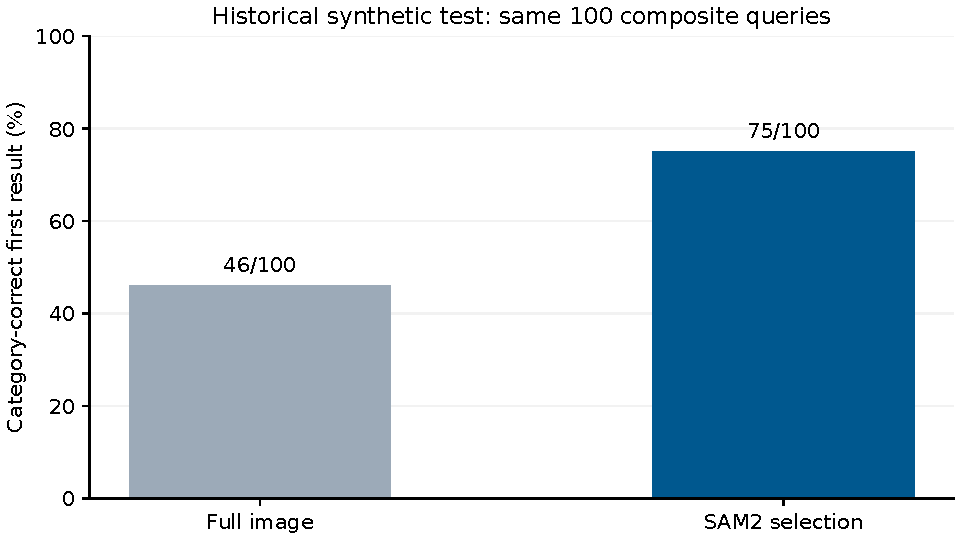
\includegraphics[width=0.96\linewidth]{images/historical_sam2.pdf}
\caption{Recorded category Top-1 on 100 synthetic test composites, not exact-product accuracy}
\label{fig:sam-historical}
\end{figure}

SAM2 corrected 39 previously incorrect first results, worsened 10, and left 51
unchanged. Thus selection helped on balance but was not beneficial on every
query. The historical validation-composite experiment recorded 48\% to 80\%
on a different set of 100 images. Its 32-point gain and the test's 29-point gain
are not competing versions of the same score and are not averaged together.

These records support a qualified conclusion: under the synthetic category
protocol, selecting the intended garment improved category retrieval compared
with representing both panels together. They do not prove that the selected
item's commercial identity was retrieved, nor do they measure the final
application's current preprocessing on a fresh independently collected dataset.

\paragraph{Application-Aligned Category Routing}
Table~\ref{tab:routing-results} and Figure~\ref{fig:routing-results} report the
separate comparison using application-prepared query embeddings and the existing
original-gallery vectors. Unrestricted and automatic search are paired on each
clean query. On test, automatic routing increases category Top-1 from 92.20\%
to 96.24\%; the gain is 4.03 percentage points after rounding the unrounded
values.

\begin{table}[H]\centering
\caption{Application-aligned clean-query category filtering comparison}
\label{tab:routing-results}
\begin{ReportTable}% Generated by generate_evidence.py; edit the source data or script.
\begin{tabular}{@{}lrrrrr@{}}
\toprule
\textbf{Split} & \textbf{$n$} & \textbf{All (\%)} & \textbf{Auto (\%)} & \textbf{Gain (pp)} & \textbf{Better / worse} \\ \midrule
Validation & 341 & 92.08 & 94.72 & 2.64 & 15 / 6 \\
Test & 372 & 92.20 & 96.24 & 4.03 & 21 / 6 \\
\bottomrule
\end{tabular}
\end{ReportTable}
\end{table}

\begin{figure}[H]\centering
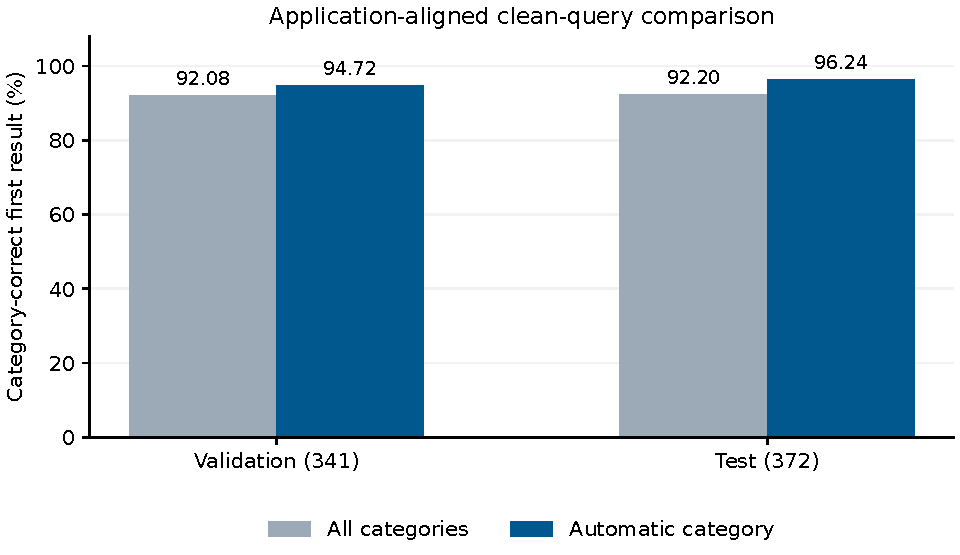
\includegraphics[width=0.96\linewidth]{images/category_routing.pdf}
\caption{Category filtering on clean validation and test queries under one application-aligned protocol}
\label{fig:routing-results}\end{figure}

The test improvement involves 21 corrected and six worsened queries. Its saved
paired 95\% bootstrap interval is $[1.34,6.72]$ percentage points, with exact
McNemar $p=0.005925$. Validation improves by 2.64 points, with interval
$[0.00,5.28]$ and $p=0.078354$. The validation result alone is not decisive at
the conventional 0.05 threshold. These figures support the retained category
filter for this clean-query task, with an explicit correction control for cases
where the category is wrong.

A later exploratory replay screened six fallback policies on the already observed
341 validation queries. Its best observed change corrected only one additional
query overall, from 323 to 324, with an interval including zero. The original
gallery's production routing was therefore left unchanged. This replay is
development analysis, not a new independent test or a justification for claiming
that the original-gallery confidence is calibrated.

\paragraph{Catalogue Cropping and the Retained Baseline}
Table~\ref{tab:crop-results} compares the original, candidate-crop, and
90\%/10\% hybrid galleries within the cropping experiment. Original-index P@1
on clean test is 92.20\%, while the crop candidate reaches 92.74\%. The gain of
0.54 points has a paired interval of $[-2.15,3.23]$ points and $p=0.845019$.
There is no reliable gain on this measure.

\begin{table}[H]\centering
\caption{Separate cropping experiment: category Top-1 within each query set}
\label{tab:crop-results}
\begin{ReportTable}% Generated by generate_evidence.py; edit the source data or script.
\begin{tabular}{@{}lrrrr@{}}
\toprule
\textbf{Query set} & \textbf{$n$} & \textbf{Original (\%)} & \textbf{Crop (\%)} & \textbf{Hybrid (\%)} \\ \midrule
Clean test & 372 & 92.20 & 92.74 & 91.94 \\
Composite: full & 100 & 48.00 & 43.00 & 49.00 \\
Composite: selected & 100 & 76.00 & 78.00 & 76.00 \\
\bottomrule
\end{tabular}
\end{ReportTable}
\end{table}

For complete composites, cropping changes P@1 from 48\% to 43\%. For selected
queries, it changes 76\% to 78\%, with an interval of $[-3,8]$ points that
includes zero. The hybrid does not provide a consistent advantage across these
sets. The decision is therefore to keep the original production index. Choosing
not to deploy an inconclusive transformation is a result of the evaluation,
not an uncompleted implementation step.

\paragraph{Reviewed Identity Pilot}
Both conditions in the forward seven-group pilot find the accepted target group
first in 7/7 queries. In the separately specified reverse comparison, full-image
and SAM2 queries also tie at 7/7 first results and MRR@10 of 1.00, with no SAM2
request failures. Each direction uses a 3,061-image gallery that excludes all
seven queries for that direction and their exact byte/pixel duplicates.

These successes show that the implemented pipeline can retrieve the reviewed
alternate views under the recorded protocol. They do not estimate general
identity accuracy: the groups were selected and visually reviewed from already
seen data, the seven groups recur in the reverse direction, and their commercial
SKU identity is unverified. With full-image Top-1 already at the ceiling, this
pilot supplies no measured SAM2 improvement. It is reported as 7/7 selected
cases, not as ``100\% system accuracy.''

\subsubsection{Discussion and Threats to Validity}
\paragraph{Catalogue Coverage and Fine-Grained Relevance}
Retrieval ranks what the catalogue contains. When the requested item is absent,
the best result can be an appropriate alternative without being the same product.
The available category labels reward type agreement and may not penalise colour,
pattern, or construction differences that matter to a visitor. A credible next
ranking study needs held-out resemblance judgments and verified identities
where exact matching is the intended task.

\paragraph{Selection and Dataset Bias}
Synthetic composites make the target explicit and keep the two garments in
separate panels. Natural outfits may involve overlap, occlusion, mixed lighting,
small garments, and people. Likewise, a successful example mask or predicted
quality score is not a segmentation benchmark. The identity pilot has a small,
purposively selected sample. Neither the synthetic experiment nor the pilot
establishes performance on a new store or independent customer-photo population.

\paragraph{Preprocessing and Historical Provenance}
The historical scripts and final application do not share every preprocessing
step. Their existence-based caches are not signed run records. The report keeps
these scores and the application-aligned comparisons separate. Fresh file hashes
and numeric consistency checks confirm the available evidence, not the missing
original execution state. No result is described as newly rerun inference merely
because its JSON was re-read during final-document verification.

\paragraph{Operational and Security Limits}
The local application has functional safeguards, but the verification is not a
penetration test, high-concurrency load test, or multi-device certification.
The final-report live tests used CPU on the same physical computer; earlier
rc.9 records include CUDA operation on that machine. No universal response-time
target is inferred from these checks. Original-gallery index operations are
locked within one process, while large public workloads would require a separate
concurrency and capacity design.

The source and runtime resources are available through the public LibaasLens
repository. Runtime publication was completed and checked on 14 November 2026:
all 28 parts and five support assets were present, and their published size/digest
records matched the local files. Anonymous download samples were checked as
recorded in \path{runtime/VERIFICATION_PUBLICATION_20261114.json}. The verified
assembled ZIP remains 1,815,578,390 bytes. These distribution checks are separate
from model accuracy and do not establish compatibility with every computer.

\subsection{User Acceptance Test}
User-acceptance evidence is the project representative's use and feedback
on the reference computer. The retained session feedback confirms interactive
selection, visually useful similar results, and the desktop launcher. The
acceptance record on 14 November 2026 confirms that the local application
works. Table~\ref{tab:acceptance-cases} records that limited scope.

\begin{table}[H]\centering
\caption{Team-representative acceptance observations and their limits}
\label{tab:acceptance-cases}
\begin{ReportTable}\begin{tabularx}{\linewidth}{@{}L{0.11\linewidth}Y Y@{}}
\toprule\textbf{ID}&\textbf{Usage scenario}&\textbf{Recorded observation}\\\midrule
UA-01 & Select an intended garment with points & The representative reported a correct selected piece and explained adding points when needed.\\\addlinespace
UA-02 & Search and inspect similar products & The representative judged some returned alternatives useful and identified less convincing rankings.\\\addlinespace
UA-03 & Start the local demonstration & The representative confirmed the desktop shortcut worked and later confirmed the application works on the team computer.\\
\bottomrule\end{tabularx}\end{ReportTable}
\end{table}

The record \path{docs/submission/TEAM_ACCEPTANCE_20261114.json} summarises the
representative's acceptance. This is informal acceptance feedback, not a
controlled multi-participant usability survey, approval by the university,
or a general accuracy measurement. No participant count, questionnaire score,
or committee signature is fabricated. The reported ranking criticism remains
a valid development observation despite successful functional acceptance.

\section{Summary}
Functional checks support the implemented local workflow, including selection,
search, administration, conflict handling, and recovery. Retrieval evidence
supports the qualified synthetic-selection result and the category-filtering
comparison, while rejecting an unsupported switch to a cropped gallery.
The identity pilot remains explicitly limited. The next chapter draws conclusions
and proposes developments consistent with those findings.
